\documentclass[a4paper,11pt]{article}
\pdfoutput=1

\usepackage[T1]{fontenc}
\usepackage[utf8]{inputenc}
\usepackage[english, swedish]{babel} %OBS! Se till att vi får rått språk.
\usepackage{amsmath}
\usepackage{lmodern}
\usepackage{helvet}
\usepackage{units}
\usepackage{icomma}
\usepackage{color}
\usepackage{graphicx}
\usepackage{bbm}
\newcommand{\N}{\ensuremath{\mathbbm{N}}}
\newcommand{\Z}{\ensuremath{\mathbbm{Z}}}
\newcommand{\Q}{\ensuremath{\mathbbm{Q}}}
\newcommand{\R}{\ensuremath{\mathbbm{R}}}
\newcommand{\C}{\ensuremath{\mathbbm{C}}}
\newcommand{\rd}{\ensuremath{\mathrm{d}}}
\newcommand{\id}{\ensuremath{\,\rd}}
\usepackage{hyperref}
\usepackage{upgreek}




%-----------------------------------------------------------------------
% Får ändras:
%-----------------------------------------------------------------------

% Öka radavståndet 1.05 / 1.2
\renewcommand{\baselinestretch}{1.05} 

\setlength{\parindent}{0cm}
\setlength{\parskip}{1.5ex}


%=======================================================================
%=======================================================================
\begin{document}

\begin{center}
 {\sf \LARGE Elektriska övningar}
\end{center}


\begin{center}
 {\sf 20--21 juni 2016}\quad {\tt v\,1.3.2}
\end{center}

\vspace{5mm} 

%------------------------------------------------------------------
% Använd endast subsection och lägre nivåer i denna dokumenttyp. 
%------------------------------------------------------------------

Syfte: Bli vän med mätinstrument, få viss vana vid kopplingar, träna 
på att skriva labbanteckningar, rita diagram, hitta enkla samband. 
 
{\sf  Tänk på:\\
Använd lagom långa sladdar.\\
Koppla in mätinstrument sist (särskilt voltmetrar).\\
Slå av spänningsaggregatet vid omkopplingar (och tänk dig för innan 
du slår på det).\\
Arbeta inte snabbare än att du hinner tänka efter vad du gör!}

\subsection*{Multimetrar}

Bekanta dig med multimetrarna.  Förklara
hur man skall göra för att med en multimeter mäta likström,
likspänning, växelström, växelspänning, resistans, 
frekvens, kapacitans. När skall 10\,A- respektive mA-kontakterna 
användas?


% \begin{figure}[h]
% 	\center
% 	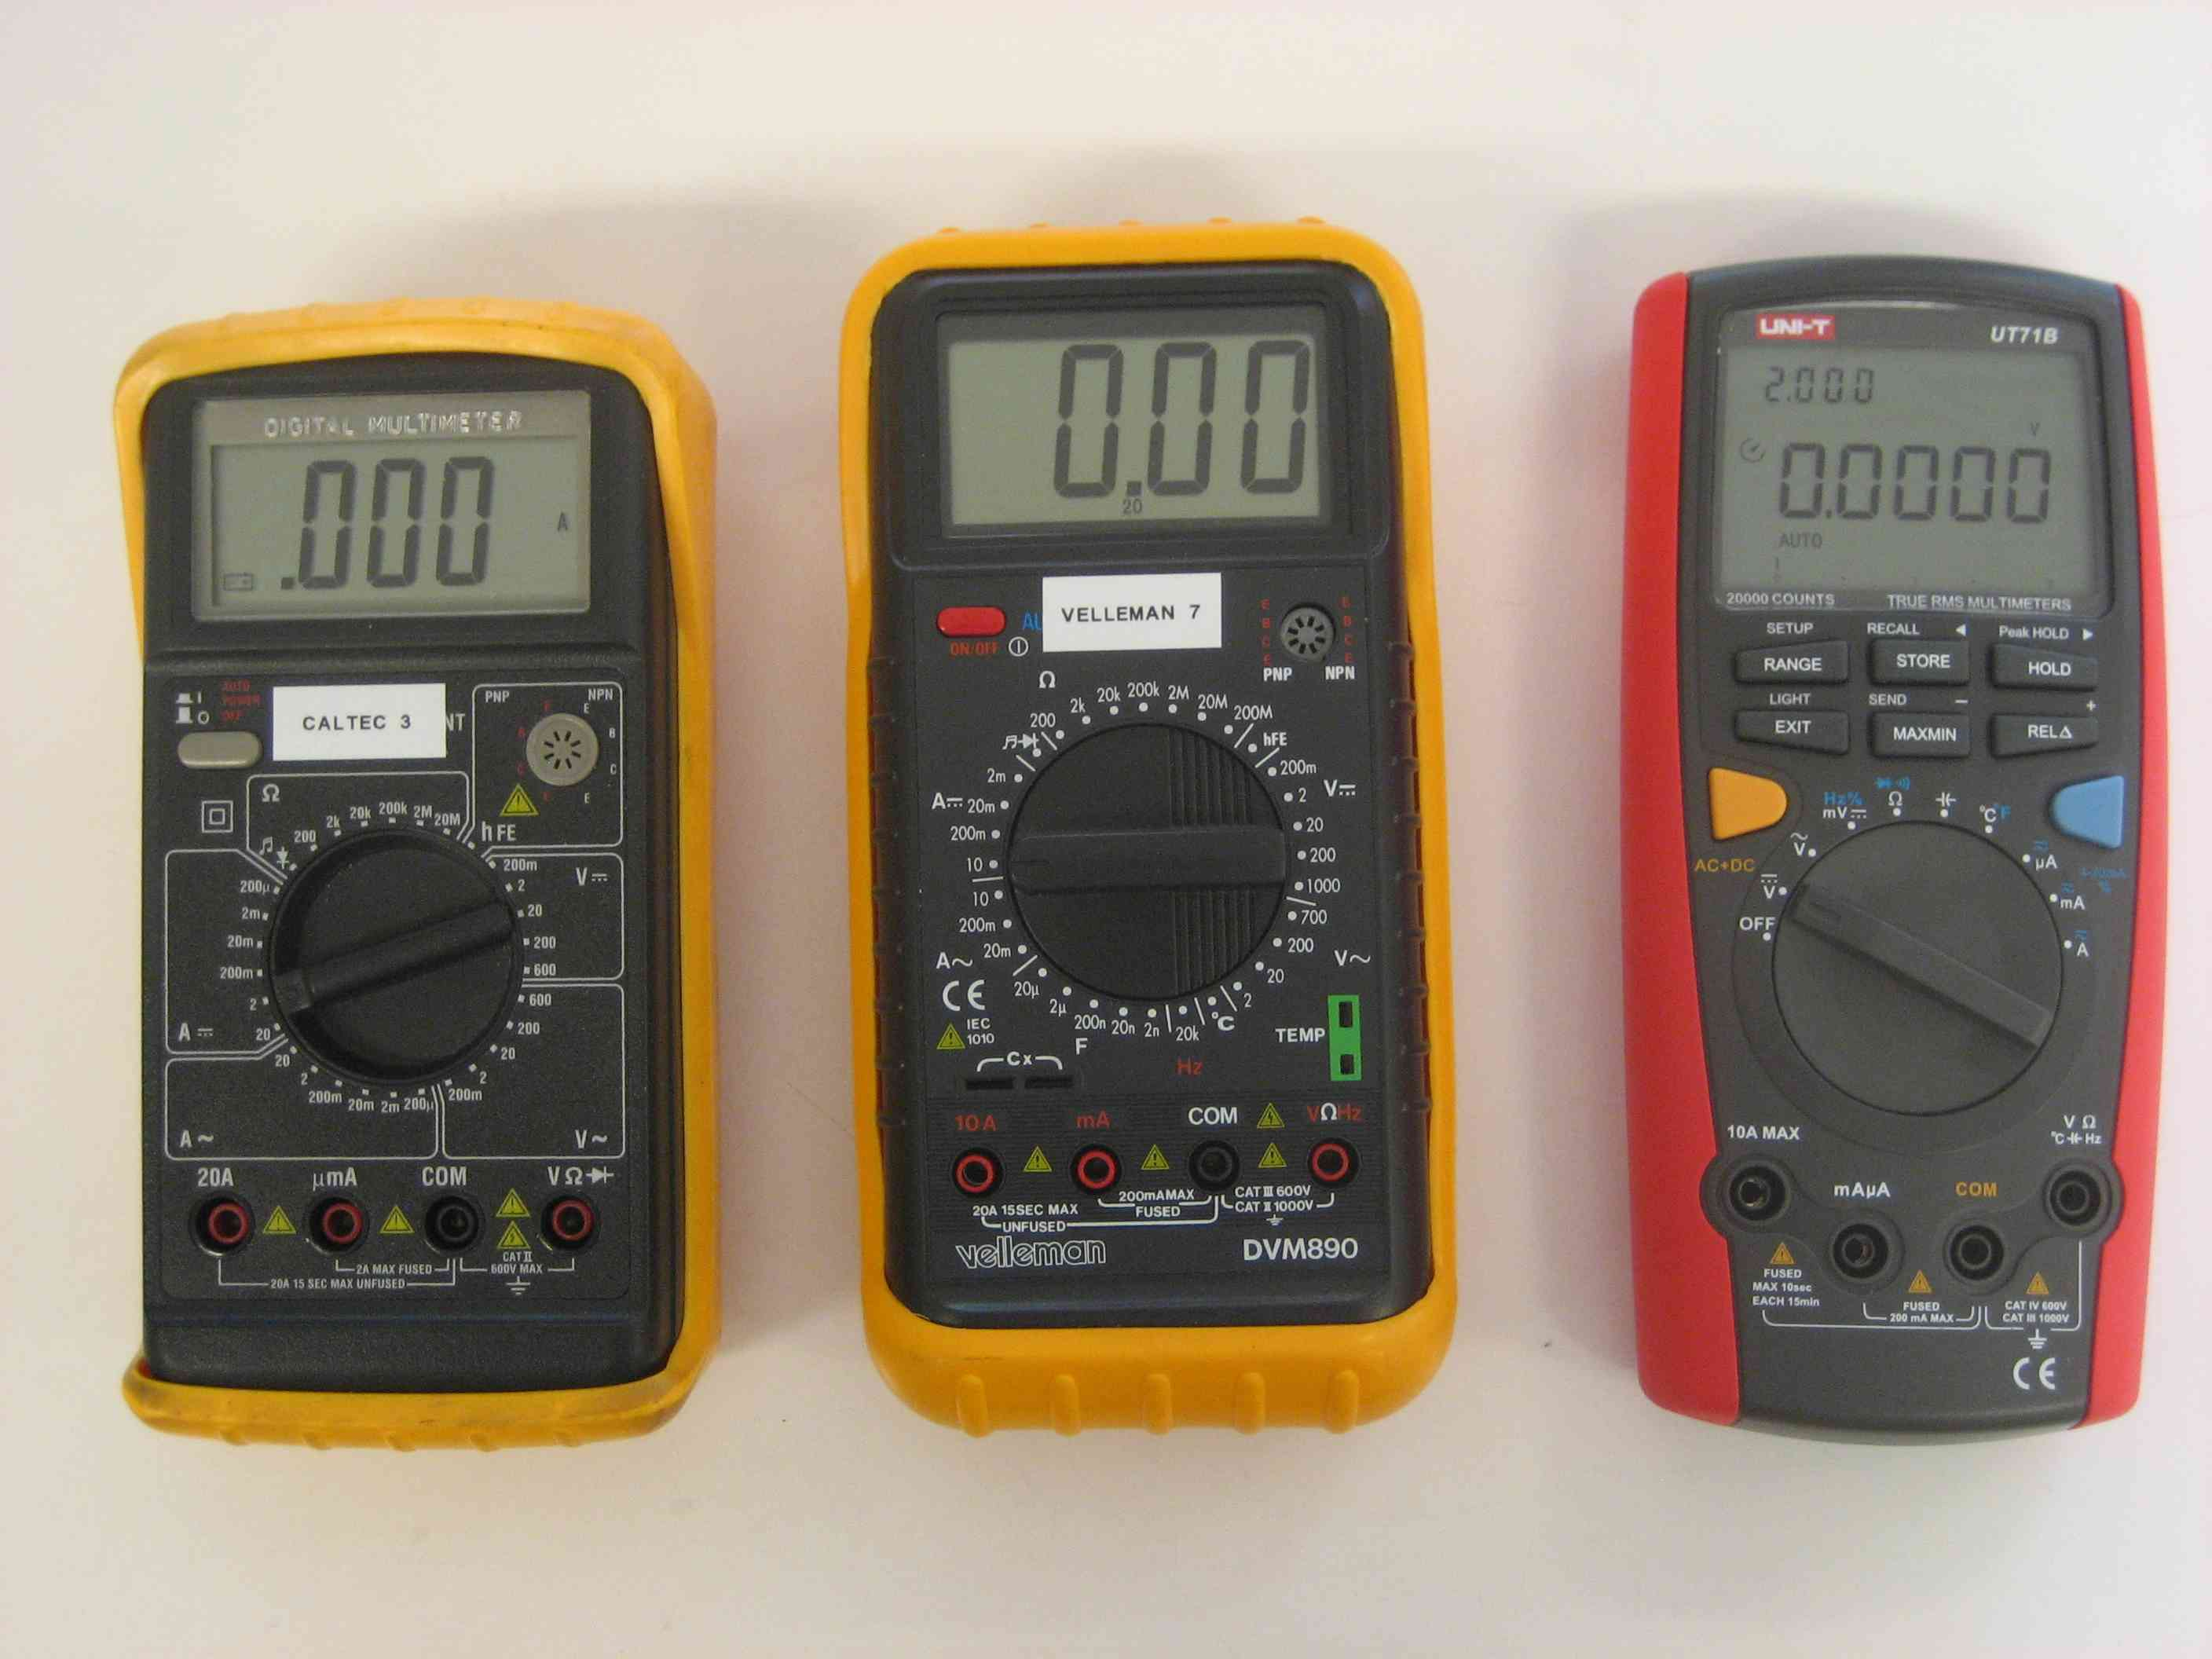
\includegraphics[width=10cm]{multim.jpg}
% % 	\caption{}
% % 	\label{}
% \end{figure}

Kan en multimeter mäta växelspänning/ström för vilka frekvenser som 
helst? Testa med funktionsgeneratorn: mät spänningen på en sinusvåg vid olika
frekvenser mellan 100\,Hz och 20\,kHz.

När multimetrar används för spännings- och strömmätningar
har de en inre resistans, vilket ibland är viktigt att vara medveten
om. Försök att mäta denna för olika mätområden (spänning och ström vid olika
känslighet). Slutsats? Hur stor ström skickar multimetern ut vid
resistansmätning? 


\subsection*{Likspänningsaggregat}

Ofta kan man välja att arbeta med strömbegränsning eller 
spänningsbegränsning. Se till att du förstår vad detta innebär.

Vad fyller jordkontakten för funktion? Prova att mäta resistansen 
mellan jordkontakterna på två olika spänningsaggregat i labsalen. 
Resultat och slutsats?

% \begin{figure}[h]
% 	\center
% 	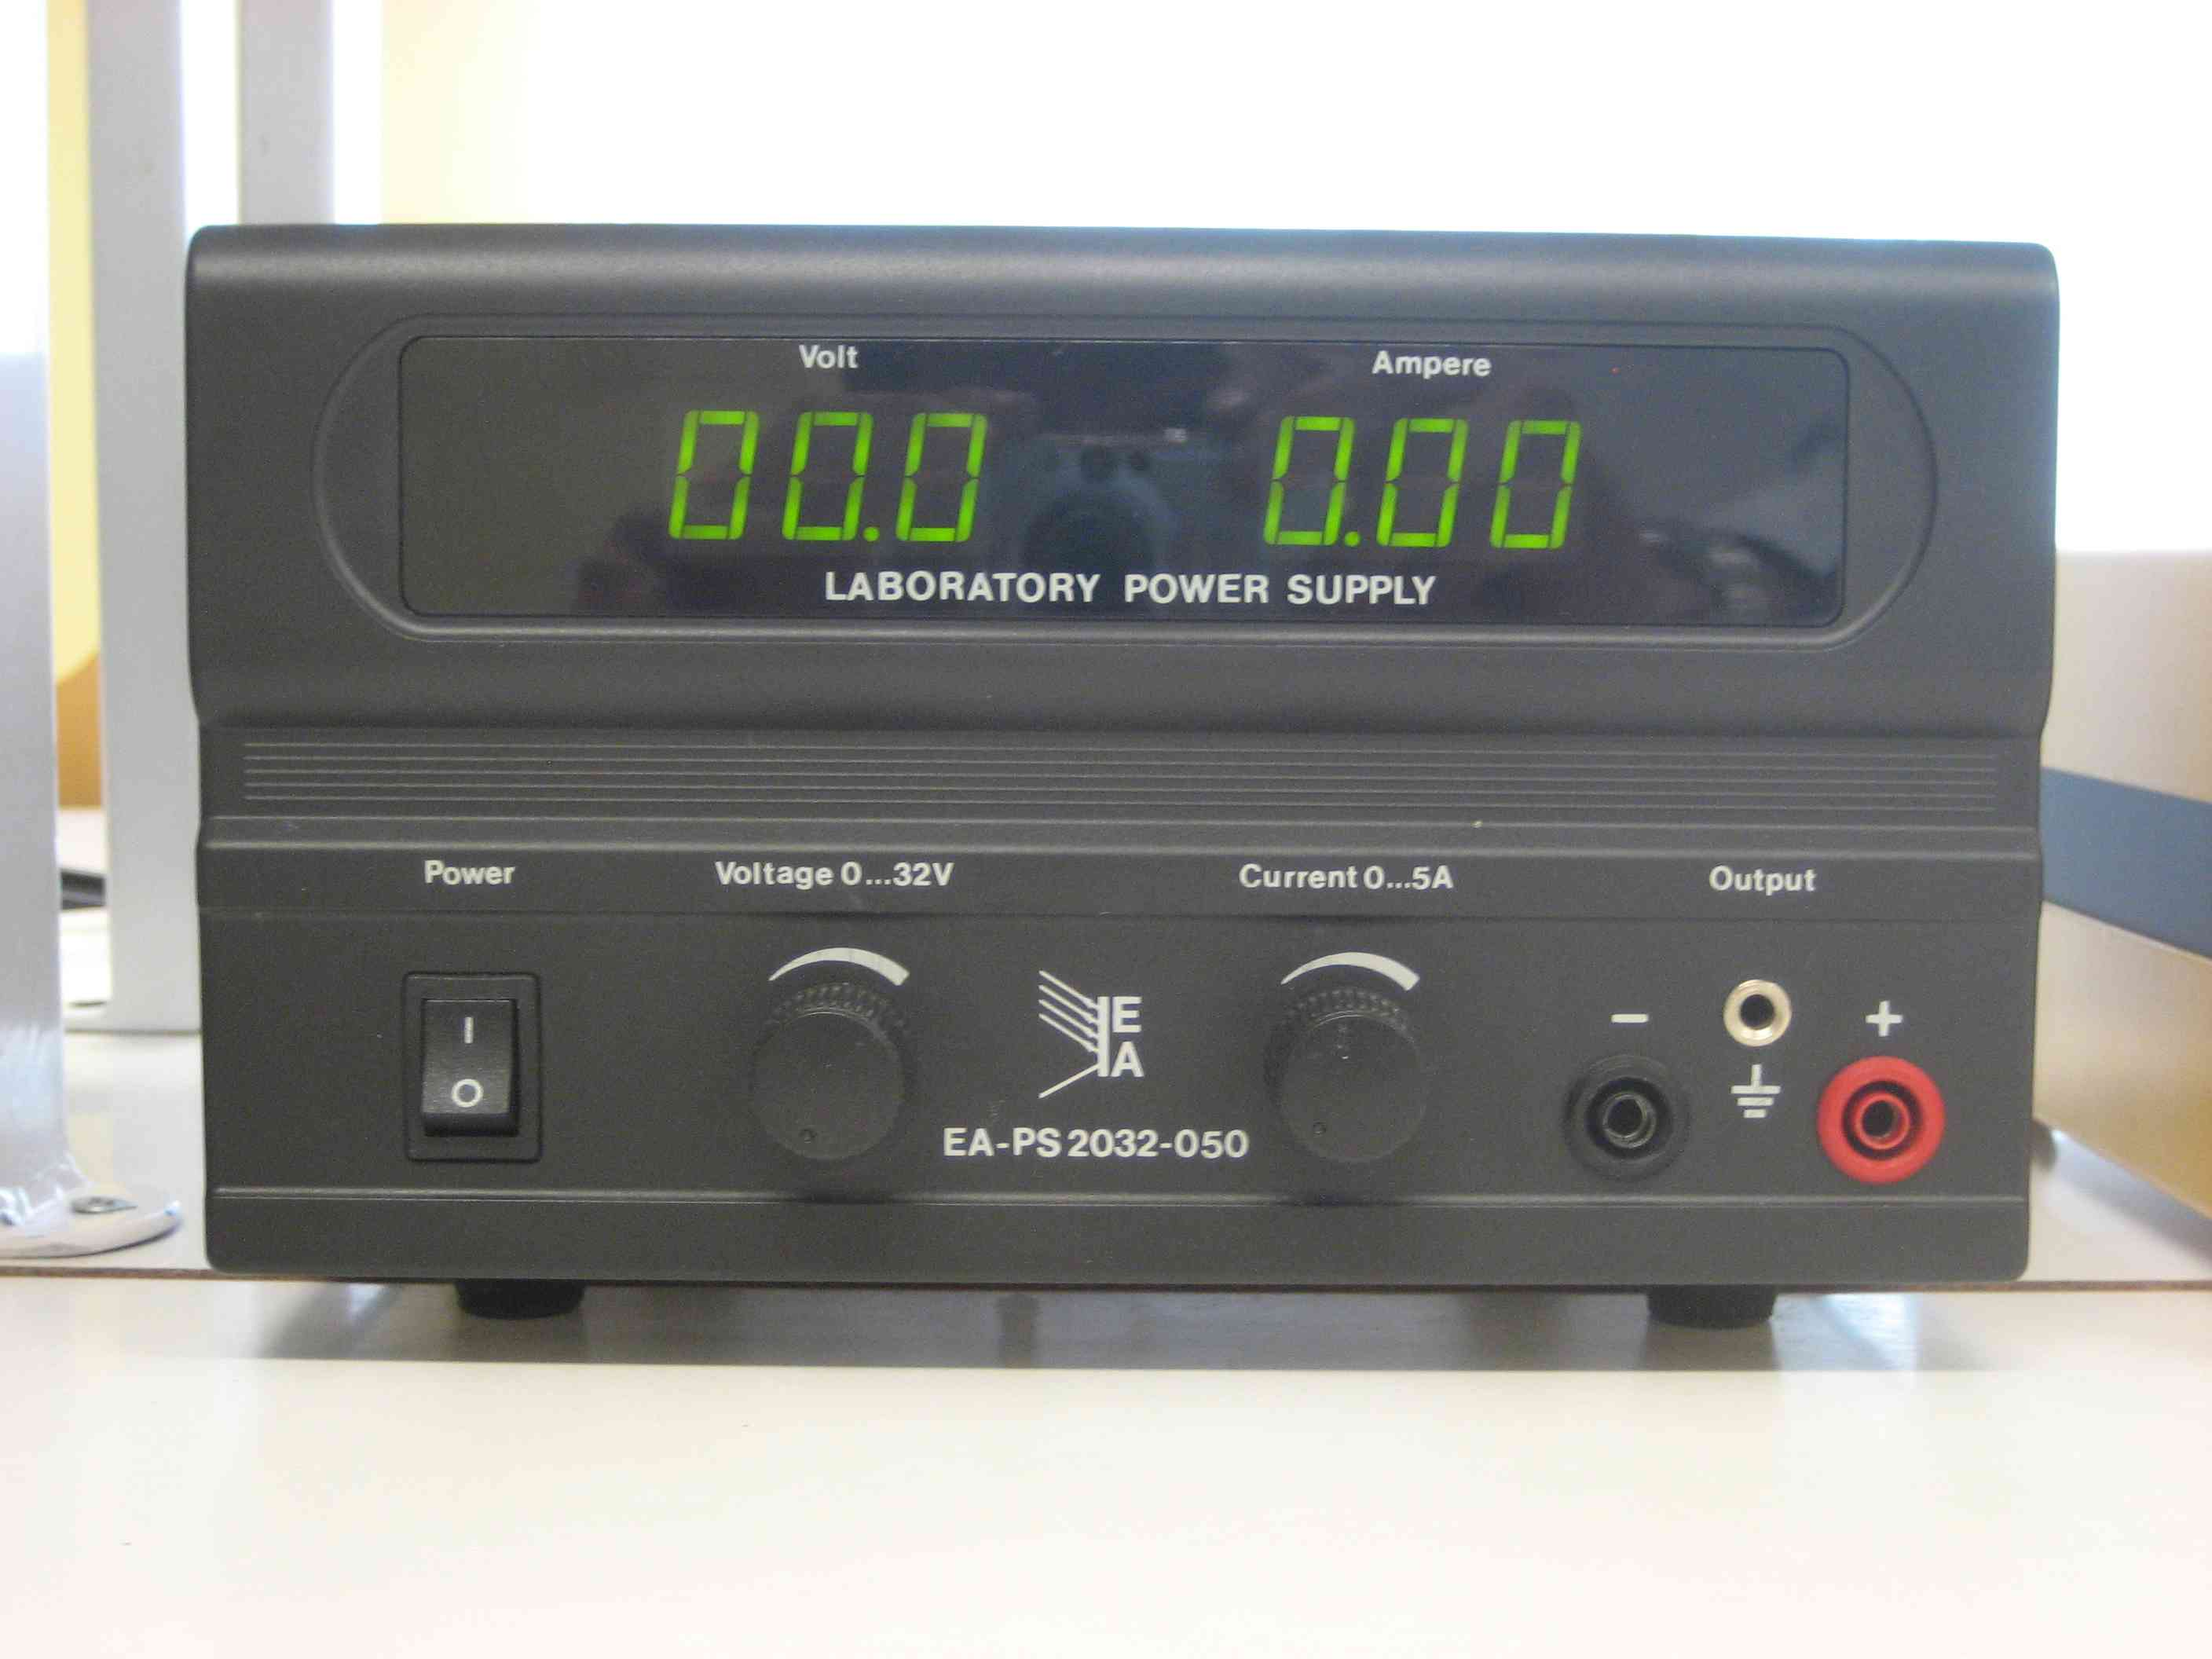
\includegraphics[width=10cm]{liksp.jpg}
% % 	\caption{}
% % 	\label{}
% \end{figure}


Hur skall man koppla om man vill ha en spänning --5\,V i förhållande 
till jord?

Kan man lita på mätinstrumenten på själva likspänningsaggregatet? 

% Gör en korrektionskurva! Det kan vara 
% lämpligt att göra en tabell enligt nedan (rätt värde = visat värde + 
% korrektion):

% \begin{tabular}{cccc}
% 	\hline
% 	Visat värde (V) & Rätt värde (V) & Felvisning (V) & 
% 	Korrektion (V)  \\
% 	\hline
% 	\ldots & \ldots & \ldots & \ldots  \\
% % 	\hline
% 	\ldots & \ldots & \ldots & \ldots  \\
% 	\hline
% \end{tabular} 




\subsection*{Mätövning: resistansmätning}

Syftet med denna övning är att göra dig uppmärksam på att man alltid 
stör när man mäter.

Vi skall arbeta med kretsen nedan, med tre olika värden på 
resistansen $R$ (se tabellen på nästa sida).

\begin{figure}[h]
	\centering
	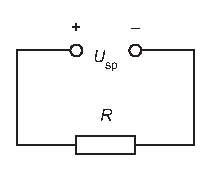
\includegraphics{fig01.eps}
% 	\caption{}
% 	\label{}
\end{figure}

Mät först respektive motstånds resistans med hjälp av 
multimeters resistansmätningsfunktion. Tänk på att motstånden inte kan vara
inkopplade i någon krets när resistansen skall mätas med ohmmeter. 

Om man skall bestämma motståndets resistans genom att mäta spänning och ström 
kan man koppla på olika sätt, se figuren nedan.

\begin{figure}[h]
	\centering
	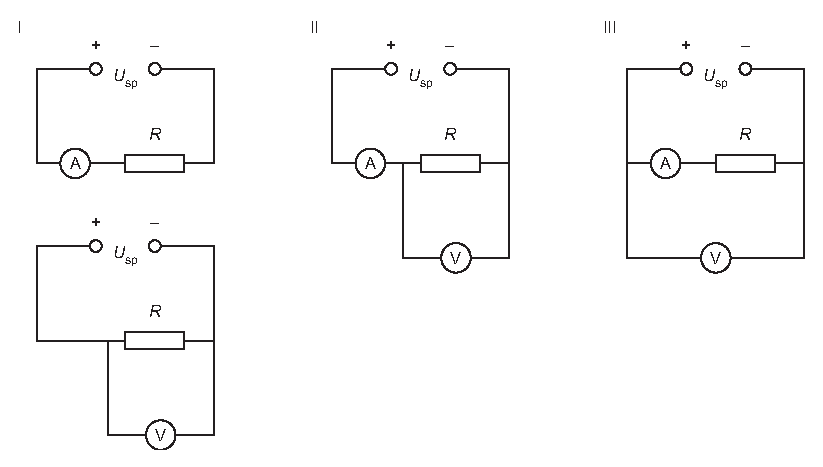
\includegraphics{fig02.eps}
% 	\caption{}
% 	\label{}
\end{figure}



Använd de olika kopplingssätten ovan för att mäta resistansen 
hos de olika motstånden. Till din hjälp finns tabellen nedan (men den är bara en
mall, gör en egen i din anteckningsbok!). Arbeta 
med ett motstånd i taget, börja med 10\,$\Upomega$ (använd inte 
högre spänningar än 1\,V för detta motstånd).

\begin{tabular}{|l|l|p{2cm}|p{2cm}|p{2cm}|}
	\hline
	& $R$ (enligt märkning) & 10\,$\Upomega$  & 10\,k$\Upomega$  & 1,0\,M$\Upomega$  \\
	\hline
	\hline
	& $R$ (mätt) &  &  &   \\
	\hline
	\hline
	& $U_{\text{sp}}$ (rekommenderat värde) & 1 V & 2 V & 15 V  \\
	\cline{2-5}
	& $U_{\text{sp}}$ (mätt) &   &   &    \\
	\cline{2-5}
	& $I$ (beräknat) &   &   &    \\
% 	\cline{2-4}
	\hline
	\hline
	I & $U$ (mätt) &   &   &    \\
	\cline{2-5}
	& $I$ (mätt) &   &   &    \\
	\cline{2-5}
	& $R$ (beräknat) &   &   &    \\
	\hline
	\hline
	II & $U$ (mätt) &   &   &    \\
	\cline{2-5}
	& $I$ (mätt) &   &   &    \\
	\cline{2-5}
	& $R$ (beräknat) &   &   &    \\
	\hline
	\hline
	III & $U$ (mätt) &   &   &    \\
	\cline{2-5}
	& $I$ (mätt) &   &   &    \\
	\cline{2-5}
	& $R$ (beräknat) &   &   &    \\
	\hline
\end{tabular} 

Kan du dra några slutsatser?

Visa hur man vid koppling II eller III kan kompensera för inre resistans i instrumenten (om 
denna är känd).

% För att få övning på att använda visarinstrument kan du göra om 
% mätningarna II och III, men med det sovjetiska visarinstrumentet 
% (U4317) istället för 
% CALTEC.

% \begin{tabular}{|l|l|p{2cm}|p{2cm}|p{2cm}|}
% 	\hline
% 	II & $U$ (mätt) &   &   &    \\
% 	\cline{2-5}
% 	& $I$ (mätt, U4317) &   &   &    \\
% 	\cline{2-5}
% 	& $R$ (beräknat) &   &   &    \\
% 	\hline
% 	\hline
% 	III & $U$ (mätt, VELLEMAN) &   &   &    \\
% 	\cline{2-5}
% 	& $I$ (mätt, U4317) &   &   &    \\
% 	\cline{2-5}
% 	& $R$ (beräknat) &   &   &    \\
% 	\hline
% \end{tabular} 

% \begin{figure}[h]
% 	\centering
% 	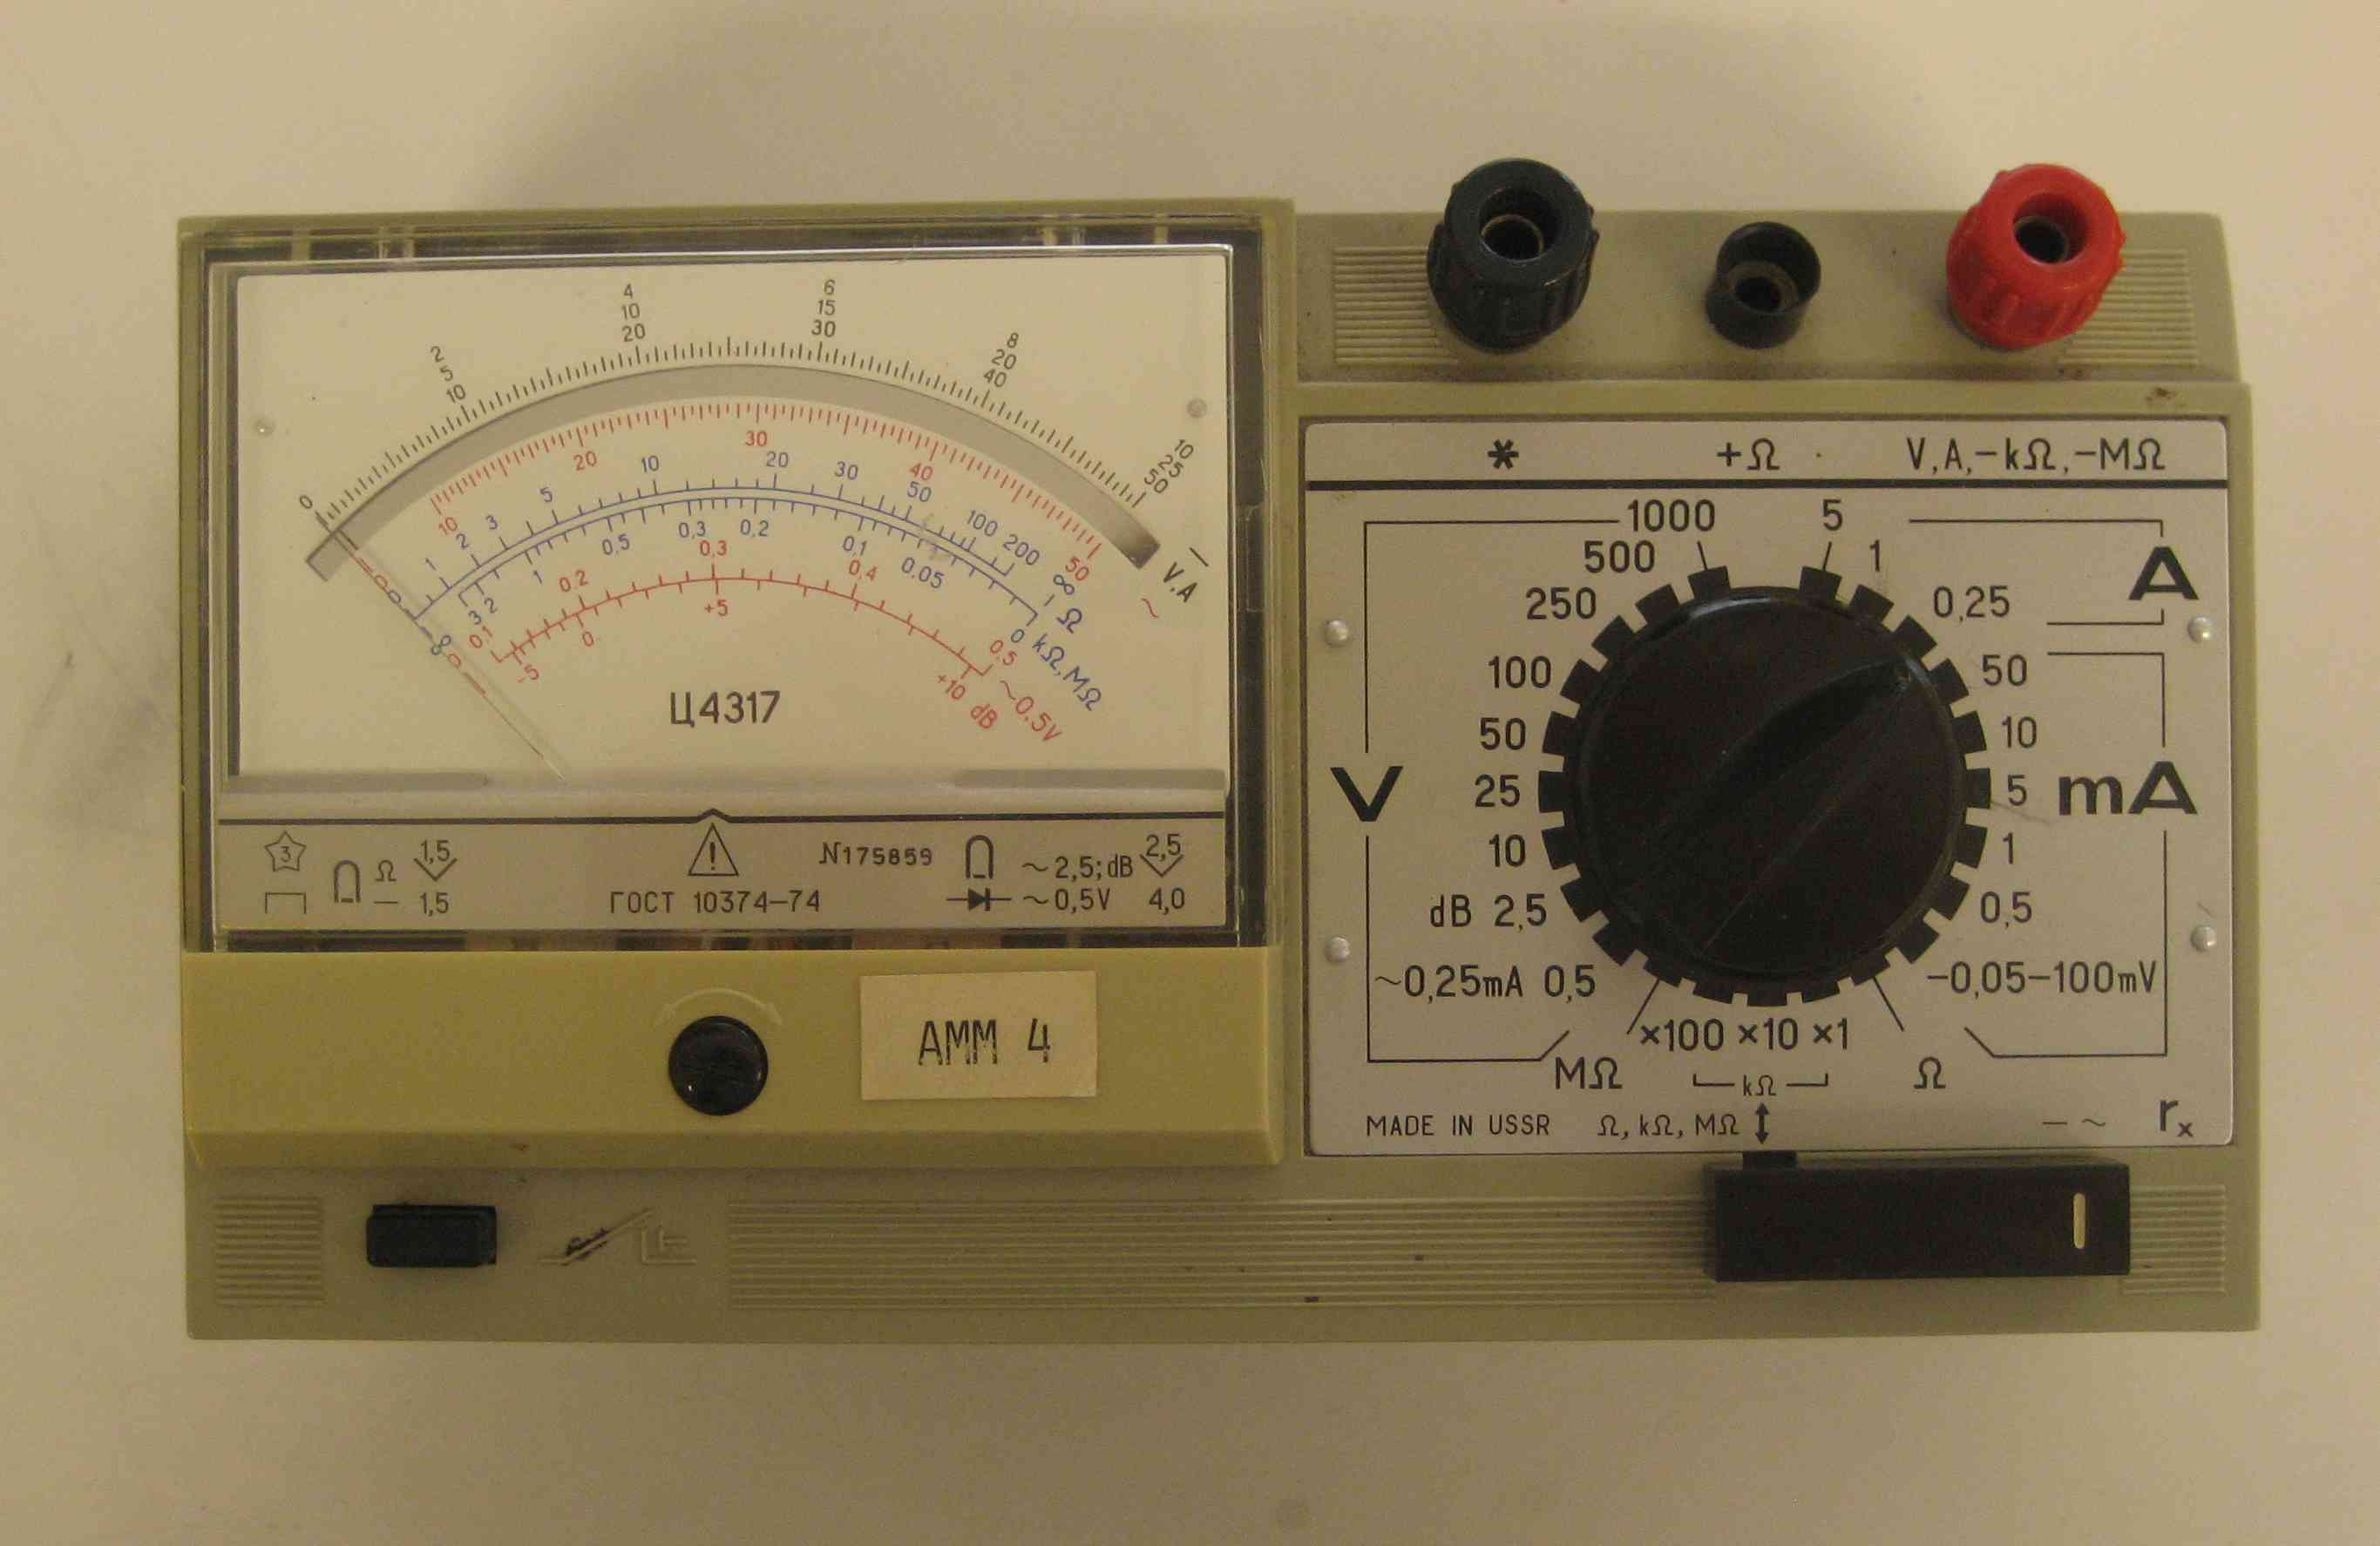
\includegraphics[width=9cm]{sovjet.jpg}
% % 	\caption{}
% % 	\label{}
% \end{figure}

\subsection*{Mätövning: spänningsdelning (om rätt materiel finns)}
Nät två resistorer kopplas i serie kommer en totala spänningen delas över
de båda resistorerna beroende på deas resistanser. 

\begin{figure}[h]
	\centering
        \resizebox{0.4\textwidth}{!}{\input{spanningsdeln.pdf_t}}
% 	\caption{}
% 	\label{}
\end{figure}

Beräkna teoretiskt hur $U_\mathrm{ut}$ beror av $U_\mathrm{tot}$, $R_x$ och
$R_\mathrm{var}$. Vad borde $U_\mathrm{ut}$ bli i specialfallen
$R_\mathrm{var}=0$ och $R_\mathrm{var}\rightarrow\infty$? Stämmer detta med vad
dina beräkningar gav?

Koppa upp kretsen ovan med ett okänt motstånd $R_x$ och använd sedan en
potentiometer som $R_\mathrm{var}$. Utnyttja nu sambandet
som du just har tagit fram för att bestämma $R_x$ (utan att behöva mäta någon
ström, men du behöver fortfarande mäta $R_\mathrm{var}$ med ohmmeter). 

Vilken är den lämpligaste inställningen på $R_\mathrm{var}$ för att
med så få beräkningar som möjligt bestämma $R_x$? Hur kan detta utnyttjas om du
ska mäta mer inveklade system?

\subsection*{Funktionsgeneratorn}

Bekanta dig med funktionsgeneratorn. Vilka typer av signaler kan den 
ge? Hur ställer man in rätt frekvens? 

Precis som allt annat har även funktionsgeneratorn en inre resistans,
$R_\mathrm{i}$. Mät den på lämpligt vis. (Notera att du endast har möjlighet att
komma åt kontakterna utanför den steckade linjen i figuren nedan.)

\begin{figure}[h]
	\centering
        \resizebox{0.4\textwidth}{!}{\input{fkngen.pdf_t}}
% 	\caption{}
% 	\label{}
\end{figure}

% \begin{figure}[h]
% 	\centering
% 	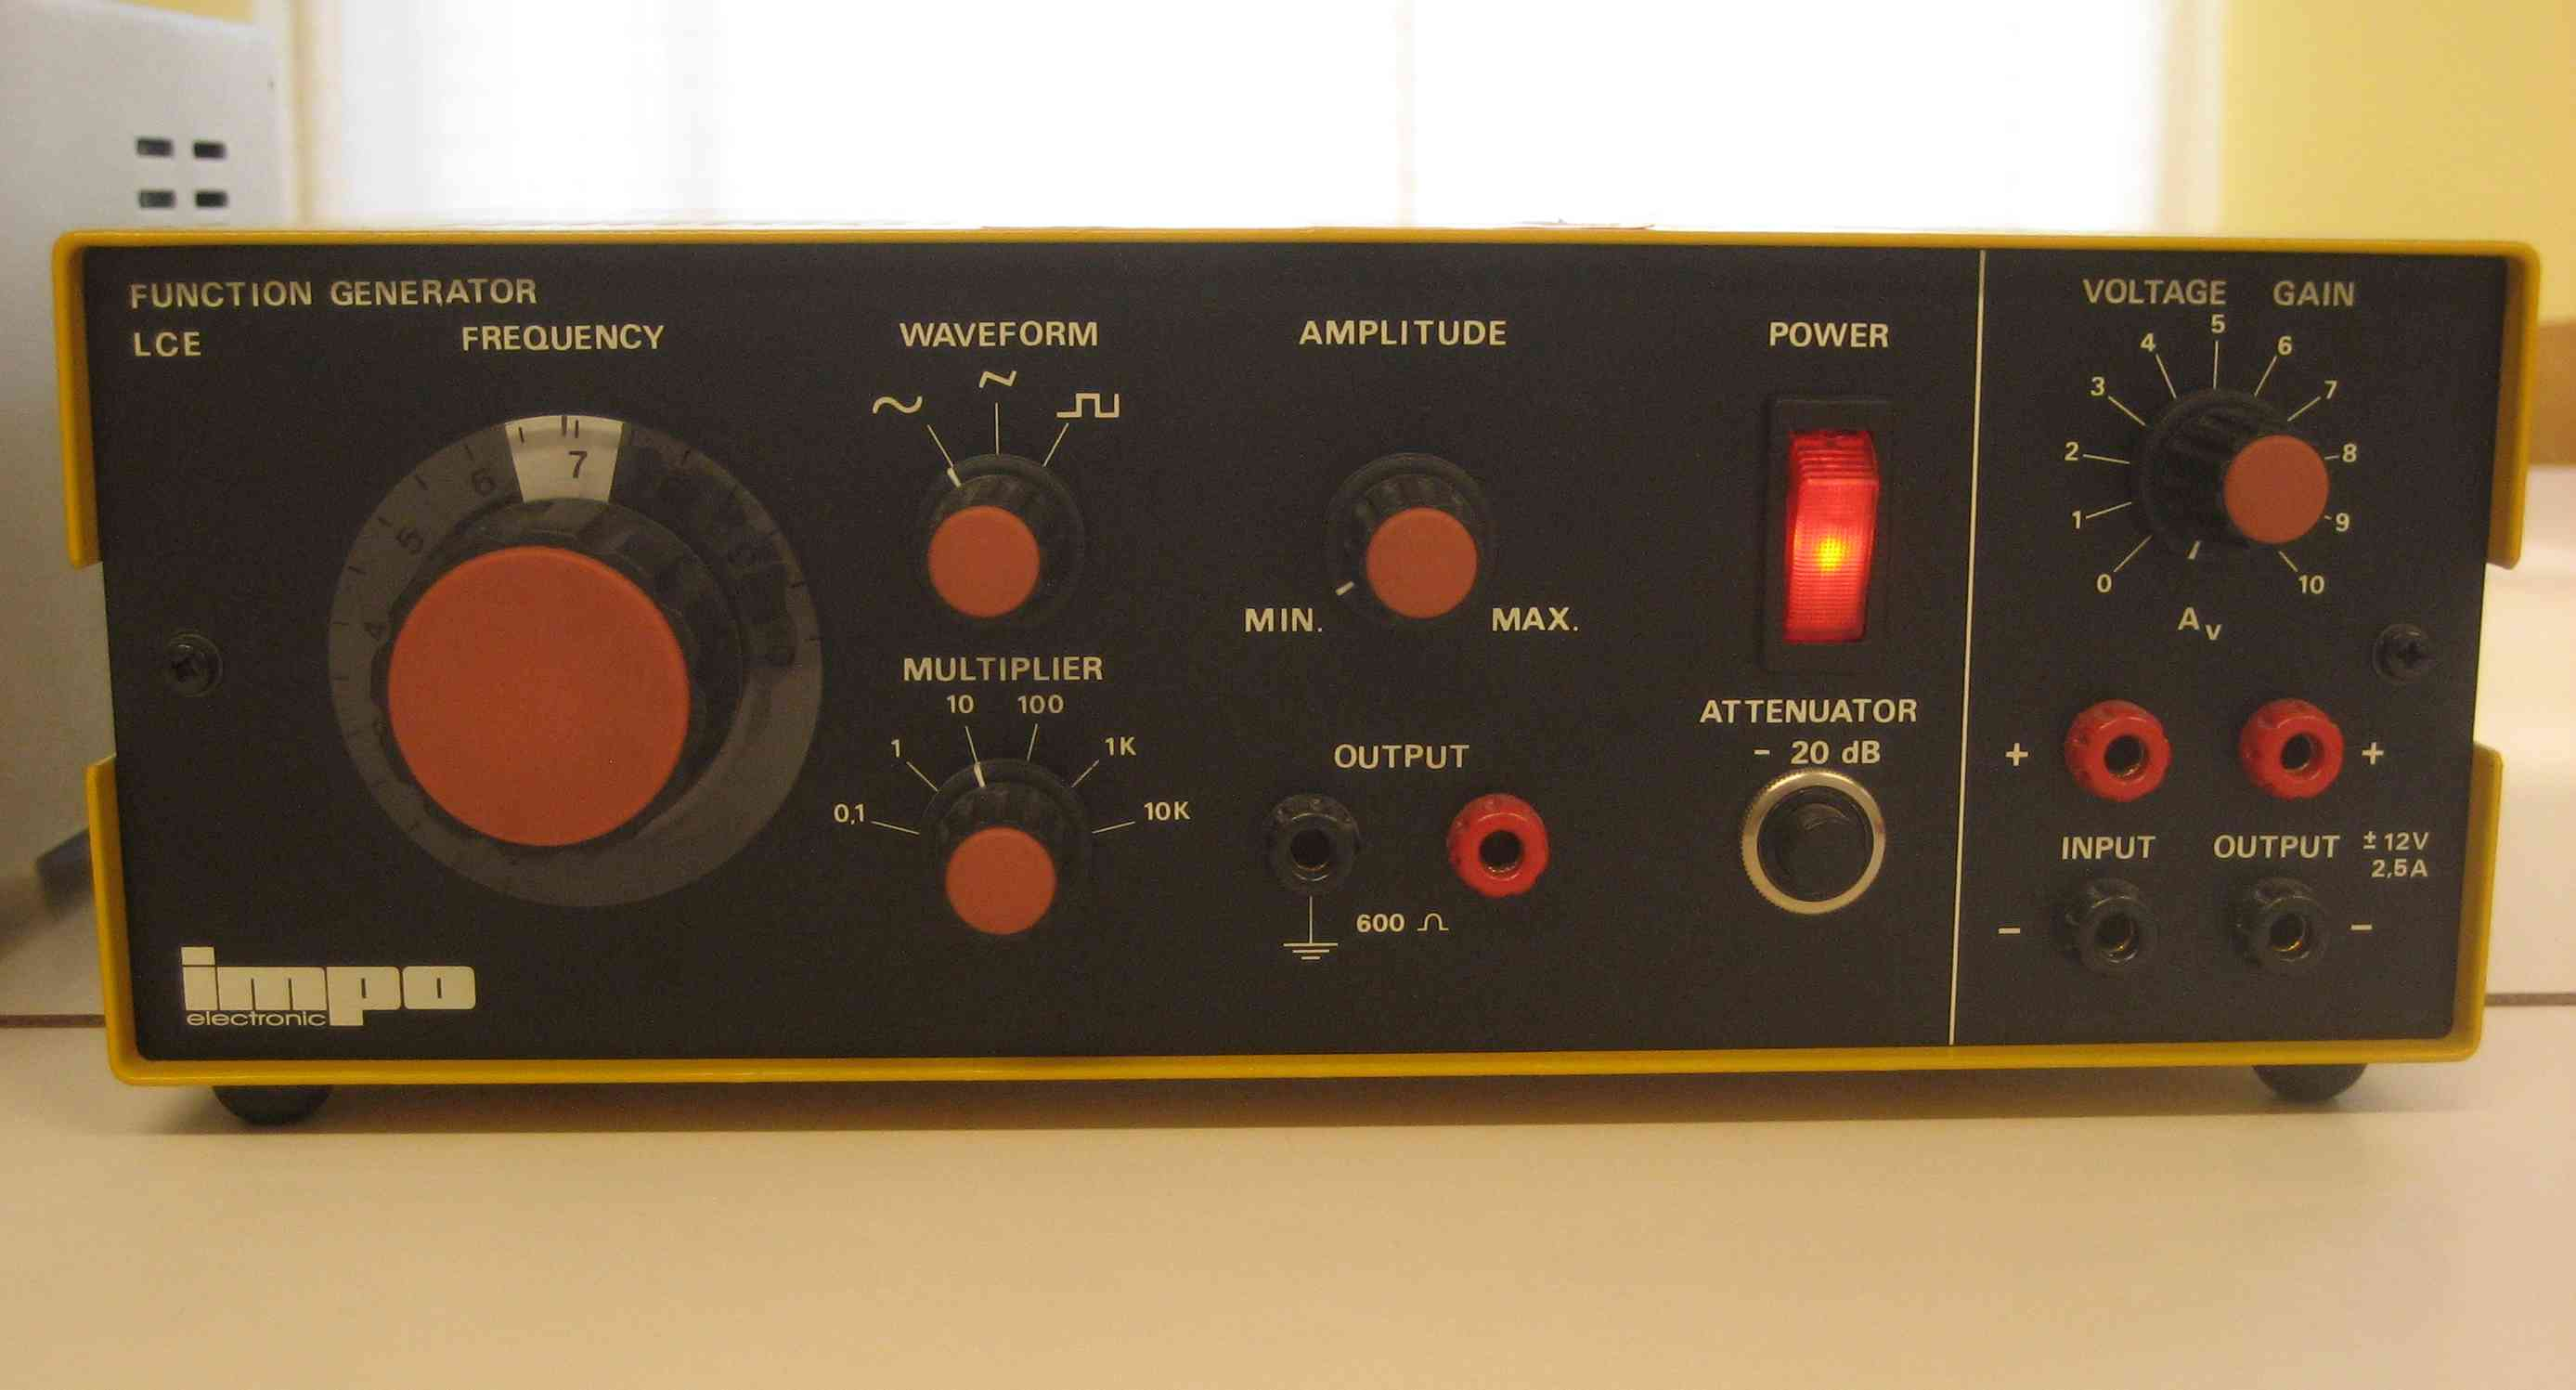
\includegraphics[width=10cm]{vaxelsp.jpg}
% % 	\caption{}
% % 	\label{}
% \end{figure}

% Koppla in en lampa och välj frekvens så att den blinkar ganska 
% långsamt (men var försiktig med 
% amplituden så att du inte bränner upp lampan). Med vilken frekvens 
% blinkar lampan (mät med stoppur)? Förklaring?


% Hur väl stämmer den verkliga frekvensen med den inställda?  
% Gör en korrektionskurva för frekvenser i intervaller 1\, kHz--10\,kHz!
% Frekvenser kan mätas med multimeter. 



% \enlargethispage{0.5cm}

\subsection*{Mätövning: reaktansens hos en kondensator}

Din uppgift är nu att  experimentellt ta fram ett samband som visar hur 
reaktansen hos en kondensator beror av frekvensen och kapacitansen.

Koppla upp en konsenstorn med ampere- och voltmeter i en yttre voltmeterkoppling
(uppkoppling~III från förra mätningen). Börja med att använda $C=1,0\,\upmu$F.

%Den eps-filen verkar inte funka
% \begin{figure}[h!]
% 	\centering
% 	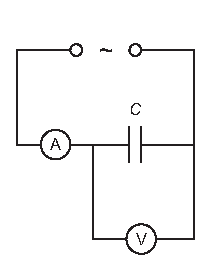
\includegraphics{fig03.eps}
% % 	\caption{}
% % 	\label{}
% \end{figure}

\emph{Samband mellan reaktans och frekvens} Bestäm reaktansen 
$X_{C}=\frac{U}{I}$ för några olika frekvenser i intervallet 20--200\,Hz. Försök
att hitta ett samband mellan reaktansen $X_{C}$ och frekvensen $f$. 

\emph{Samband mellan reaktans och kapacitans} Håll frekvensen konstant
och bestäm reaktansen för några olika värden på kapacitansen $C$ (hur
kan du variera $C$ om du endast har tillgång till 1,0\,$\upmu$F och 
2,2\,$\upmu$F-kondensatorer?).  Försök att hitta ett samband mellan
reaktansen $X_{C}$ och kapacitansen $C$.

Sätt samman de båda delsambanden ovan till ett samband och bestäm 
proportionalitetskonstanten med felgränser. Om du vill kan du jämföra med det teoretiska resultatet.





\subsection*{Mätövning: reaktansens hos en spole (om tiden tillåter)}
%\textcolor{red}{Våra multimetrar klarar inte av att mäta vid så höga frekvenser. Så om vi ska göra den här uppgiften måste vi ha bättre utrustning.}

Gör om samma undersökning som ovan fast med spole (10\,mH, flera kan 
seriekopplas) istället för 
kondensator.  Lämpliga frekvenser: 1--10\,kHz. Använd oscilloskopen för att mäta ström och spänning. Hur mäter man ström med ett oscilloskop.

\subsection*{Mätövning: resonans}
%\textcolor{red}{Det kanske blir för mycket för dem att ta med $\mathrm{j}\omega$-metoden för dem också.}

Du ska här mäta spänningen över motståndet i de olika kretsarna nedan som
funktion av frekvensen på inspänningen. Koppla upp en krets i taget. Välj
$L=\unit[20]{mH}$, $C=\unit[3,2]{\upmu F}$ och $R=\unit[10]{k\Upomega}$. Finns
det några max./min. hos $u_R$ i de olika kretsarna? Om såfall vid vilken frekvens? Hur ser det ut i specialfallen $\omega = 0$ och $\omega \rightarrow \infty$?

\begin{figure}[h]
	\centering
        \resizebox{0.65\textwidth}{!}{\input{resonans.pdf_t}}
% 	\caption{}
% 	\label{}
\end{figure}



% \subsection*{Oscilloskopet}
% 
% Se först till att du förstår principen för hur ett oscilloskop 
% fungerar (se till exempel ``13.8 Oscilloskopet'' från gamla Alphonce)
% 
% \enlargethispage{0.6cm}
% 
% \begin{figure}[h]
% 	\includegraphics[width=12cm]{osc.jpg}
% % 	\caption{}
% % 	\label{}
% \end{figure}
% 
% Slå på oscilloskopet och undersök reglagen\\ {\sf 
% TIME/DIV} 
% (tidbasratten)\\ {\sf INTEN}\\ {\sf FOCUS}
% 
% Vad har tidbasratten för funktion?
% 
% 
% 
% \subsection*{Koaxialkablar}
% 
% Innan vi går vidare kan det vara bra att tänka efter hur 
% koaxialkablar och BNC-kontakter fungerar. Hur ser en koaxialkabel ut 
% i genomskärning? Klipp inte upp, använd istället Wikipedia eller nåt liknande!
% 
% En viktig sak att tänka på 
% är att den svarta banankontakten är kopplad till höljet på 
% BNC-kontakten, som blir jordad när BNC-kontakten ansluts till ett 
% oscilloskop. Testa gärna att mäta resistansen mellan de svarta 
% bananstiften på två koaxialkablar kopplade till varsitt oscilloskop, 
% eller resistansen mellan jordkontakten på likspänningsaggregatet och 
% det svarta bananstiftet på koaxialkabel ansluten till oscilloskop. 
% Vad händer om du drar ur nätsladden till endera apparaten?
% 
% \subsection*{Mätövning: Lyssna på och mät sinussignaler}
% 
% Koppla en högtalare till funktionsgeneratorn, och mät spänningen över 
% högtalaren med oscilloskopet (fråga om du vill ha hjälp med 
% oscilloskopinställningar så här i början).
% 
% \begin{figure}[h]
% 	\centering
% 	\includegraphics{fig04.eps}
% % 	\caption{}
% % 	\label{}
% \end{figure}
% 
% 
% Undersök oscilloskopets reglage (relevanta först nu när mätsignal är
% inkopplad)\\
% {\sf VOLTS/DIV}\\
% {\sf AC GND DC}
% 
% Om du vill kan du också testa {\sf TRIGGER}-reglagen.
% 
% Gör en lista med de steg man bör gå igenom för att ställa in 
% oscilloskopet.
% 
% 
% 
% 
% Tillbaka till funktionsgeneratorn.  ändra signalens frekvens och
% amplitud och beskriv vad du ser och hör.
% 
% 
% Ställ in valfri frekvens och amplitud. Mät frekvensen och 
% toppspänningen med oscilloskop. Mät också spänningens effektivvärde 
% och frekvens med multimeter (VELLEMAN eller UNI-T, kolla att 
% multimetern klarar av att mäta vid frekvensen ifråga). Stämmer 
% mätningarna överens? 
% 
% 
% Hur höga frekvenser kan örat uppfatta? (Finns det någon lurighet här?)
% 
% Går det att mäta den undre gränsen också?
% 
% 
% 
% 
% \subsection*{Mätövning: Spännings- och strömmätning med oscilloskop}
% 
% Oscilloskopet kan bara mäta spänning, men genom att mäta spänningen 
% över ett motstånd med liten resistans $R$ kan ström mätas indirekt 
% (eftersom $i=\frac{u}{R}$).
% 
% Koppla upp enligt nedan. Använd 1 kHz, ca  2 V topp-till-topp 
% sinussignal.
% 
% 
% 
% \begin{figure}[h]
% 	\centering
% 	\includegraphics{fig05.eps}
% % 	\caption{}
% % 	\label{}
% \end{figure}
% 
% Mät spänningen över motstånden 
% på CH1 och strömmen på CH2. Tänk efter så att du inte kortsluter via 
% jordkontakterna. Trigga på strömsignalen (hur gör du detta?).
% 
% % \thispagestyle{empty}
% 
% \newpage
% 
% Rita av oscilloskopbilden. Gör också ett diagram som visar hur 
% spänningen och strömmen varierar med tiden (gradera axlarna korrekt).
% 
% \begin{figure}[h!]
% 	\centering
% 	\includegraphics{osc_rutor.eps}
% % 	\caption{}
% % 	\label{}
% \end{figure}
% 
% Antag att vi vill  mäta spänningen över 470 $\Upomega$-motståndet 
% enbart. Om man kopplar som i figuren nedan blir det galet. Förklara 
% varför! Hur skall man bära sig åt för att det skall bli rätt?
% 
% \begin{figure}[h]
% 	\centering
% 	\includegraphics[width=3cm]{fig06.eps}
% % 	\caption{}
% % 	\label{}
% \end{figure}
% 
% 
% \subsection*{Mätövning: Likriktning av växelström med diod}
% 
% Koppla upp enligt nedan. Använd 1 kHz, ca 2 V topp-till-topp 
% sinussignal. Trigga på CH1.
% 
% \begin{figure}[h]
% 	\centering
% 	\includegraphics{fig07.eps}
% % 	\caption{}
% % 	\label{}
% \end{figure}
% 
% 
% Rita av oscilloskopskärmen och förklara vad du ser. Vad kan en diod 
% användas till?
% 
% \begin{figure}[h]
% 	\centering
% 	\includegraphics{osc.eps}
% % 	\caption{}
% % 	\label{}
% \end{figure}
% 
% Titta på båda signalerna samtidigt. Rita och förklara vad du ser.
% 
% 
% 
% 
% \subsection*{Mätövning: Upp- och urladdning av kondensator}
% 
% 
% 
% Koppla upp en RC-krets enligt figuren nedan. Välj fyrkantvåg från 
% funktionsgeneratorn.
% 
% \begin{figure}[h]
% 	\centering
% 	\includegraphics{fig08.eps}
% % 	\caption{}
% % 	\label{}
% \end{figure}
% 
% 
% Man kan teoretiskt visa att tiden det tar för en kondensator att 
% laddas ur till hälften ges av
% \[
% 	t_{1/2}=RC \ln 2.
% \]
% Visa detta (se avsnitt 31.7 i boken)!
% 
% Rita av oscilloskopskärmen och förklara vad du ser.
% 
% \begin{figure}[h]
% 	\centering
% 	\includegraphics{osc.eps}
% % 	\caption{}
% % 	\label{}
% \end{figure}
% 
% Mät $t_{1/2}$ (bestäm felgränser) och jämför med teoretiska 
% värdet. Se till att välja frekvens så att kondensatorn hinner 
% laddas ur/upp.
% 
% Gör mätningar och beräkningar för några olika värden på resistansen 
% $R$ (10 k$\Upomega$, 22 k$\Upomega$, 33 k$\Upomega$).
% 
% 
% 
% \subsection*{Mätövning: Enkla växelströmskretsar}
% 
% Koppla upp enligt figuren nedan. Använd VELLEMAN som frekvensmätare, 
% och två stycken UNI-T som ampere- och voltmeter. De senare kan mäta 
% upp till 10 kHz, så undvik högre frekvenser. Trigga på CH2 (strömmen).
% 
% \begin{figure}[h]
% 	\centering
% 	\includegraphics{fig09.eps}
% % 	\caption{}
% % 	\label{}
% \end{figure}
% 
% 
% \newpage
% 
% {\bf Spänning och ström i krets med enbart resistans}
% 
% Kortslut spole och kondensator. Rita kopplingsschema
% 
% \begin{figure}[h]
% 	\includegraphics{kopplschema.eps}
% % 	\caption{}
% % 	\label{}
% \end{figure}
% 
% 
% Mät spänning $U$ och ström $I$  med multimetrar.
% 
% $U =$ \rule[-1mm]{15mm}{0.5pt} 
% 
% $I =$ \rule[-1mm]{15mm}{0.5pt}
% 
% Stämmer dessa mätvärden överens med avläsningar på oscilloskopet?
% 
% $\hat{u} =$  \rule[-1mm]{15mm}{0.5pt}  ger $U =$ \rule[-1mm]{15mm}{0.5pt} 
% 
% $\hat{i} =$  \rule[-1mm]{15mm}{0.5pt}  ger $I =$ \rule[-1mm]{15mm}{0.5pt}
% 
% 
% Rita av oscilloskopbilden och gör ett visardiagram (i 
% effektivvärdesskala).
% 
% \begin{figure}[h]
% 	\centering
% 	\includegraphics{osc_rutor.eps}
% % 	\caption{}
% % 	\label{}
% \end{figure}
% 
% \newpage
% 
% {\bf Spänning och ström i krets med enbart kapacitans}
% 
% 
% \enlargethispage{1cm}
% 
% Kortslut spole och motståndet $R$. Om frekvensen $f$ väljs så att 
% $1/(2\pi f C) \gg R_{1}$ kommer kretsen att uppföra sig som en ideal 
% kondensator.
% 
% Rita kopplingsschema.
% 
% \begin{figure}[h]
% 	\includegraphics{kopplschema.eps}
% % 	\caption{}
% % 	\label{}
% \end{figure}
% 
% Mät spänning $U$ och ström $I$ och frekvens $f$ med multimetrar:
% 
% $U =$ \rule[-1mm]{15mm}{0.5pt} 
% 
% $I =$ \rule[-1mm]{15mm}{0.5pt}
% 
% $f$  = \rule[-1mm]{15mm}{0.5pt} ger $X_{C}=\frac{1}{2\pi f C} =$ 
% \rule[-1mm]{15mm}{0.5pt} 
% 
% \hfill och $U = X_{C}I = \frac{I}{2\pi f C}=$ 
% \rule[-1mm]{15mm}{0.5pt}.
% 
% 
% Stämmer dessa mätvärden överens med avläsningar på oscilloskopet?
% 
% $\hat{u} =$  \rule[-1mm]{15mm}{0.5pt}  ger $U =$ \rule[-1mm]{15mm}{0.5pt} 
% 
% $\hat{i} =$  \rule[-1mm]{15mm}{0.5pt}  ger $I =$ \rule[-1mm]{15mm}{0.5pt}
% 
% $T =$  \rule[-1mm]{15mm}{0.5pt}  ger $f$ \rule[-1mm]{15mm}{0.5pt}
% 
% Bestäm fasförskjutningen med oscilloskopet. 
% 
% $\varphi = $ \rule[-1mm]{15mm}{0.5pt}
% 
% 
% Rita av oscilloskopbilden och gör ett visardiagram (i 
% effektivvärdesskala).
% 
% \begin{figure}[h]
% 	\centering
% 	\includegraphics{osc_rutor.eps}
% % 	\caption{}
% % 	\label{}
% \end{figure}
% 
% I en ren kapacitans ligger alltså spänningen fasförskjuten  
% \rule[-1mm]{15mm}{0.5pt} före/efter strömmen (stryk det som ej gäller).
% 
% 
% \newpage
% 
% {\bf Spänning och ström i krets med enbart induktans}
% 
% \enlargethispage{1cm}
% 
% Kortslut kondensatorn och motståndet $R$. Om frekvensen $f$ väljs så att 
% $2\pi f L \gg R_{1}$ kommer kretsen att uppföra sig som en ideal 
% induktans.
% 
% Rita kopplingsschema.
% 
% \begin{figure}[h]
% 	\includegraphics{kopplschema.eps}
% % 	\caption{}
% % 	\label{}
% \end{figure}
% 
% 
% Mät spänning $U$ och ström $I$ och frekvens $f$ med multimetrar:
% 
% $U =$ \rule[-1mm]{15mm}{0.5pt} 
% 
% $I =$ \rule[-1mm]{15mm}{0.5pt}
% 
% $f$  = \rule[-1mm]{15mm}{0.5pt} ger $X_{L}=2\pi f L =$ 
% \rule[-1mm]{15mm}{0.5pt} 
% 
% \hfill och $U = X_{L}I = I\cdot 2\pi f L=$ 
% \rule[-1mm]{15mm}{0.5pt}.
% 
% 
% Stämmer dessa mätvärden överens med avläsningar på oscilloskopet?
% 
% $\hat{u} =$  \rule[-1mm]{15mm}{0.5pt}  ger $U =$ \rule[-1mm]{15mm}{0.5pt} 
% 
% $\hat{i} =$  \rule[-1mm]{15mm}{0.5pt}  ger $I =$ \rule[-1mm]{15mm}{0.5pt}
% 
% $T =$  \rule[-1mm]{15mm}{0.5pt}  ger $f$ \rule[-1mm]{15mm}{0.5pt}
% 
% Bestäm fasförskjutningen med oscilloskopet. 
% 
% $\varphi = $ \rule[-1mm]{15mm}{0.5pt}
% 
% 
% Rita av oscilloskopbilden och gör ett visardiagram (i 
% effektivvärdesskala).
% 
% \begin{figure}[h]
% 	\centering
% 	\includegraphics{osc_rutor.eps}
% % 	\caption{}
% % 	\label{}
% \end{figure}
% 
% 
% I en ren induktans ligger alltså spänningen fasförskjuten  
% \rule[-1mm]{15mm}{0.5pt} före/efter strömmen (stryk det som ej gäller).
% 
% 
% \newpage
% 
% {\bf Spänning och ström i krets med  induktans och resistans i 
% serie}
% 
% 
% 
% 
% Kortslut nu enbart kondensatorn och justera frekvensen så att $U_{R}$ 
% är jämförbar med $U_{L}$. (Spänningen $U_{R_{1}}$ kan antas vara 
% försumbar.)
% 
% Rita kopplingsschema.
% 
% \begin{figure}[h]
% 	\includegraphics{kopplschema.eps}
% % 	\caption{}
% % 	\label{}
% \end{figure}
% 
% 
% Mät  med multimetrar:
% 
% $U =$ \rule[-1mm]{15mm}{0.5pt} 
% 
% $U_{L} =$ \rule[-1mm]{15mm}{0.5pt}
% 
% $U_{R} =$ \rule[-1mm]{15mm}{0.5pt}
% 
% $I =$ \rule[-1mm]{15mm}{0.5pt}
% 
% $f$  = \rule[-1mm]{15mm}{0.5pt} 
% 
% Rita visardiagram för resistans och induktans i serie (i 
% effektivvärdesskala, strömmen riktvisare). Du kan utgå från att 
% $u_{L}(t)$ och $u_{R}(t)$ är fasförskjutna 90$^{\circ}$.
% 
% \begin{figure}[h]
% 	\centering
% 	\includegraphics{rutor.eps}
% % 	\caption{}
% % 	\label{}
% \end{figure}
% 
% 
% 
% Mätning i figuren ger   $U =$ \rule[-1mm]{15mm}{0.5pt}  och  
% $\varphi =$ \rule[-1mm]{15mm}{0.5pt}
% 
% Mätning på oscilloskopet ger fasförskjutningen $\varphi =$ \rule[-1mm]{15mm}{0.5pt}
% 
% Beräkna också $U$ och $\varphi$ från angivna värden på $R$ och $L$ 
% och mätta värden på $f$ och $I$ (se boken avsnitt 37.3).
% 
% 
% 
% 
% 
% \newpage
% 
% {\bf Spänning och ström i krets med  kapacitans och resistans i 
% serie}
% 
% 
% 
% Kortslut nu enbart induktansen och justera frekvensen så att $U_{R}$ 
% är jämförbar med $U_{C}$. (Spänningen $U_{R_{1}}$ kan antas vara 
% försumbar.)
% 
% Rita kopplingsschema.
% 
% \begin{figure}[h]
% 	\includegraphics{kopplschema.eps}
% % 	\caption{}
% % 	\label{}
% \end{figure}
% 
% Mät  med multimetrar:
% 
% $U =$ \rule[-1mm]{15mm}{0.5pt} 
% 
% $U_{C} =$ \rule[-1mm]{15mm}{0.5pt}
% 
% $U_{R} =$ \rule[-1mm]{15mm}{0.5pt}
% 
% $I =$ \rule[-1mm]{15mm}{0.5pt}
% 
% $f$  = \rule[-1mm]{15mm}{0.5pt} 
% 
% Rita visardiagram för resistans och induktans i serie (i 
% effektivvärdesskala, strömmen riktvisare). Du kan utgå från att 
% $u_{C}(t)$ och $u_{R}(t)$ är fasförskjutna 90$^{\circ}$.
% 
% \begin{figure}[h]
% 	\centering
% 	\includegraphics{rutor.eps}
% % 	\caption{}
% % 	\label{}
% \end{figure}
% 
% Mätning i figuren ger   $U =$ \rule[-1mm]{15mm}{0.5pt}  och  
% $\varphi =$ \rule[-1mm]{15mm}{0.5pt}
% 
% Mätning på oscilloskopet ger fasförskjutningen $\varphi =$ \rule[-1mm]{15mm}{0.5pt}
% 
% Beräkna också $U$ och $\varphi$ från angivna värden 
% på $R$ och $C$ 
% och mätta värden på $f$ och $I$ (se boken avsnitt 37.3).
% 
% \newpage
% 
% \subsection*{Mätövning: Serieresonans}
% 
% Återgå till kretsen med resistans $R$, induktans $L$ och 
% kapacitans $C$ i serie.
% 
% 
% Variera frekvensen och studera på oscilloskopet  hur ström- och 
% spänningskurvorna förskjuts då kretsen är omväxlande induktiv ($X_{L} 
% >  X_{C}$), rent resistiv (($X_{L} 
% = X_{C}$ och kapacitiv ($X_{L} 
% <  X_{C}$. Leta sedan upp resonansfrekvensen, det vill säga den 
% frekvens som ger största värdet på strömmen $I$. 
% 
% Mät  med multimetrar:
% 
% $U =$ \rule[-1mm]{15mm}{0.5pt} 
% 
% $U_{L} =$ \rule[-1mm]{15mm}{0.5pt}
% 
% $U_{C} =$ \rule[-1mm]{15mm}{0.5pt}
% 
% $U_{R} =$ \rule[-1mm]{15mm}{0.5pt}
% 
% $I =$ \rule[-1mm]{15mm}{0.5pt}
% 
% $f$  = \rule[-1mm]{15mm}{0.5pt} 
% 
% Rita visardiagram.
% 
% \begin{figure}[h]
% 	\centering
% 	\includegraphics{rutor.eps}
% % 	\caption{}
% % 	\label{}
% \end{figure}
% 
% Beräkna också den teoretiska resonansfrekvensen från angivna värden 
% på $R$ och $C$ (se boken avsnitt 36.7, 37.3).
% 
% 
% \subsection*{Mätövning: Resonanskurva}
% 
% Koppla upp en krets med $C=100$ nF och $L=100$ mH i serie och mät upp 
% en resonanskurva liknande bokens figur 36-13.
% 
% [Mer detaljerade instruktioner?]

\subsection*{Mätövning: Linjärisering}

Sista övningen blir att öva på linjärisering. Du får fyra stycken 
motståndstrådar med samma längd och av samma
material, men med olika tvärsnittsareor. Din uppgift är att bestämma materialets
resistivitet så noggrant som möjligt. 

Vi noterar att den mätta resistansen kan skrivas
\[
R = R_{0}+\frac{\rho l }{A} = R_{0} + \rho l \frac{1}{A}
\]
där $R_{0}$ är resistans i mätsladdar och kontakter. Nu ser vi att om 
vi ritar $R$  som funktion av $\frac{1}{A}$ så förväntar vi oss en 
rät linje med lutningen $\rho$, som kan bestämmas grafiskt. Genom att sedan mäta
$l$ kan $\rho$ beräknas. 

Gör mätningar och analys för att bestämma resistiviteten (med 
felgräns)!



% \newpage
% 
% \thispagestyle{empty}
% 
% \begin{figure}[h]
% 	\includegraphics{oscSTOR.eps}
% % 	\caption{}
% % 	\label{}
% \end{figure}






\end{document}
%=======================================================================



%------------------------------------------------------------------
% Enkel referens i text:  
%------------------------------------------------------------------
\ldots se till exempel
\emph{Hur universum fick sina fläckar} av Levin (Norstedts, Stockholm, 2003)


%------------------------------------------------------------------
% Exempel på headers:  
%------------------------------------------------------------------
Icke-euklidisk geometri {\footnotesize (v.\ 1.0)}
Kursinformation Ma AB

%------------------------------------------------------------------
% 2\,000
%------------------------------------------------------------------
